\chapter{Resultados}
\label{chap:Result}

	Neste capítulo será apresentado o método utilizado, os resultados obtidos durante
	o desenvolvimento deste estudo conforme a \cref{fig:fluxogramaProposta},o qual
	apresenta as fases: definição da linguagem de programação e das características
	a serem extraídas; códigos-fontes; extração de características; mineração de dados e
	agrupamento; e projeção e visualização. A linguagem de programação escolhida foi \texttt{Python},
	as características serão originadas pela análise estática e do estilo de escrita,
	os códigos-fontes consiste em duas base de dados distintas, a extração
	de características ocorreu por meio de ferramentas disponibilizadas livremente, a
	mineração e agrupamento dos dados foi realizada utilizando a similaridade do
	cosseno, enquanto a projeção e a visualização dos dados foi realizada pela ferramenta
	\texttt{Science View}.
	 % TODO: mencionar que este capítulo é uma instância do método apresentado no capítulo anterior, considerando as fases XYZ. Explique em uma linha o que foi feito para cada fase.
	 
	\section{\foreign{Science View}}
		A ferramenta \foreign{Science View} \cite{Alencar} foi desenvolvida para exibir
		as relações entre os documentos dado um acervo de artigos científicos, utilizando
		a \acs{T-LSP} a partir de artigos nos formatos \foreign{ISI}, \foreign{Endnote Export Format}
		ou \foreign{BibTeX}.
		
		A fim de criar uma nova projeção multidimensional dinâmica, a ferramenta guia o usuário
		para: inserir um novo conjunto de documentos ou utilizar uma coleção presente no banco
		de dados; definir parâmetros sobre o pré-processamentos dos dados e a redução de
		dimensionalidade; decidir qual ténica de projeção e o cálculo de distância a ser utilizado;
		e determinar os parâmetros referente a \acs{T-LSP}.


 	\section{Método}
	 	Após a revisão da literatura, verificamos que o projeto é baseado em algumas etapas.
	 	Conforme a \cref{fig:fluxogramaProposta}, é necessário escolher qual linguagem de programação
	 	será utilizado. Em seguida deve-se verificar quais características podem ser extraídas
	 	das implementações submetidas utilizando a linguagem especificada. Posteriormente, é
	 	necessário construir a base de dados por meio da submissão de implementações, realizar
	 	a extração de características, minerar os dados extraídos das submissões e verificar a
	 	similaridade entre as implementações. Por fim, realizar a projeção e visualizar os
	 	agrupamentos.
	 	
	 	\begin{figure}[h]
	 		\centering
	 		\includegraphics[width=0.7\linewidth]{imagem/fluxogramaProposta}
	 		\caption{Fluxograma das etapas necessárias para a realização do projeto}
	 		\label{fig:fluxogramaProposta}
	 	\end{figure}
	 	
	 	A \textbf{linguagem de programação} refere-se a definição de qual linguagem será
	 	utilizada para o desenvolvimento do projeto. Por exemplo: \texttt{C}, \texttt{Java}
	 	ou \texttt{Python}. Deve ser escolhida conforme a demanda da sua utilização, pela
	 	disponibilidade de cursos de programação ofertado em \acs{MOOC}s ou pelo conhecimento de
	 	ferramentas que possam verificar características dessa linguagem, como o
	 	\texttt{cpplint} para a linguagem \texttt{C}, \texttt{Checkstyle} para
	 	\texttt{Java} e \texttt{PEP8} para \texttt{Python}.
	 	
	 	A etapa seguinte \textbf{definir características a serem extraídas} será realizado
	 	com base nos trabalhos relacionados (\cref{sec:TrabRel}). Verificamos que é
	 	possível utilizar características originadas de um tipo de análise (estática,
	 	dinâmica e do estilo de escrita), bem como associar características de análises
	 	distintas para obter um melhor resultado.
	 	
	 	O estágio \textbf{códigos-fontes} refere-se à construção da base de dados que será
	 	utilizada no experimento. Tal base tem que possuir uma quantidade considerável de
	 	submissões de códigos-fontes, devido a quantidade de usuários que utilizam o \acs{MOOC},
	 	para que seja possível avaliar o desenvolvimento do projeto com uma quantidade
	 	condizente com o número de usuários.
	 	
	 	A \textbf{extração de características} é a fase na qual escolhe-se uma ferramenta
	 	disponibilizada livremente pela Internet que forneça os dados necessários, visto
	 	que não desejamos criar uma ferramenta para esse fim. Tal estágio é responsável pela
	 	adaptação das ferramentas selecionadas anteriormente para que seja possível obter
	 	as características e salvá-la em algum tipo de arquivo, como o formato \texttt{XML}
	 	e o \texttt{CSV}, por exemplo.
	 	
	 	Na etapa \textbf{mineração de dados e agrupamento} analisa-se os dados obtidos a
	 	fim de verificar um padrão das características obtidas. Isso permite a utilização
	 	de técnicas para verificar a similaridade dos códigos-fontes a fim
	 	de produzir os agrupamentos.
	 	
	 	Por fim, \textbf{projeção e visualização} refere-se ao emprego de técnicas de
	 	projeção para que seja possível diminuir a quantidade de dimensões. Uma dimensão
	 	é referente a uma característica extraída da implementação, portanto a quantidade
	 	de dimensões é igual a quantidade de características extraídas. Com isso, é
	 	necessário selecionar uma técnica para diminuir um espaço n-dimensional para
	 	duas ou três dimensões a fim de realizar a visualização dos agrupamentos.
	 	
	 	No caso das características extraídas não forem relevantes para a formação de
	 	agrupamentos ou a visualização não produzir modelos gráficos significativos por
	 	meio dos mapeamento de dados realizados pela técnica de projeção, será necessário
	 	voltar a segunda etapa para definir outras características a serem extraídas.
	 	
	 	Nosso objetivo, por meio dessas etapas, consiste no desenvolvimento de subsídios
	 	de avaliação, utilizando técnicas de visualização para auxiliar os professores a
	 	corrigirem todas as submissões, considerando o tempo e a qualidade do \foreign{feedback},
	 	principalmente. Por isso, teremos três questões de pesquisa (QP):
	 	
	 	\begin{itemize}
	 		\item \textbf{QP$_1$}: o algoritmo de agrupamento produz grupos de códigos-fontes
	 		com boa qualidade?
	 		\item \textbf{QP$_2$}: a utilização de subsídios de avaliação reduz o tempo % TODO: retirar tempo e abordar isso nas conclusões como trabalhos futuros
	 		de correção de todas as submissões?
	 	\end{itemize}
	 	
	 	O subsídio de avaliação será uma adaptação da \texttt{Science View} \cite{Alencar-etal:2012}
	 	que, originalmente, verifica as mudanças nas relações de documentos com o decorrer do tempo,
	 	utilizando técnicas de mineração, projeção e visualização. Com isso, teremos as
	 	seguintes hipóteses (HP) em relação a utilização da proposta deste estudo:
	 	
	 	\begin{itemize}
	 		\item \textbf{HP$_1$}: tempo para corrigir os exercícios com os subsídios é inferior  % TODO: mudar esta hipótese para avaliar a qualidade da visualização
	 		ao tempo necessário com a correção manual;
	 	\end{itemize}
	 	
	 	Para validar o tempo gasto e a qualidade dos \texttt{feedbacks} para todas as correções,
	 	será criado dois grupos de professores. Um grupo utilizou a técnica proposta nessa pesquisa para
	 	realizar a avaliação das implementações, enquanto o outro grupo avaliou as submissões
	 	manualmente. Além disso, a qualidade dos \foreign{feedbacks}, será avaliado através de \foreign{survey}
	 	e questionário para cada aluno sobre o \foreign{feedback} que recebeu e também será avaliado
	 	por meio de submissões futuras, visto que a ferramenta realiza várias projeções ao longo do tempo.

	\section{Definição da linguagem de programação}
		Foi definido a utilização da linguagem de programação Python. A escolha foi
		devido ao conhecimento prévio de ferramentas que possam auxiliar na verificação
		e extração de características, bem como a disponibilidade de cursos sobre
		introdução a programação, utilizando \texttt{Python}, em diversos \acs{MOOC}s.

	\section{Definição das características a serem extraídas}
		Considerando a combinação de características originadas de tipos de análises
		distintas, utilizamos uma combinação de aspectos provenientes da análise  % TODO: a banca apresentou dúvidas o que seriam tais características. Isso é sinal de que precisamos melhor a descrição do capítulo 2. Além disso, parte das informações apresentads na seção "Extração de características" deve vir pra cá (não é necessário colocar partes sobre ferramenta utilizada, mas precisamos informar que foram selecionadas as características de quantidades de linhas de código, complexidade ciclomática e quantidade de violações de regras de estilo de escrita definida pelo PEP8).
		estática e do estilo de escrita. A escolha da análise estática se dá pela
		possibilidade de implementações para solucionar o mesmo problema possuírem
		o mesmo tamanho. Enquanto a organização do código, realizado pelo programador,
		pode impactar no entendimento da solução do problema, por isso a escolha da
		análise do estilo de escrita. Para isso, utilizaremos a ferramenta \texttt{Flake8}
		\cite{flake8} que pode adquirir todas as características necessárias por meio da
		utilização de \foreign{plugins}. Não utilizaremos a análise dinâmica pela falta
		de conhecimento de ferramentas que nos forneça tal característica e pelo pouco
		tempo hábil para implementação de uma ferramenta para realizar esse tipo de
		análise e validação dessa ferramenta.
		
		As características a serem extraídas da análise estática serão apenas a quantidade
		de linhas de código e a complexidade ciclomática da implementação. Em relação
		a análise do estilo de escrita, será considerado todas as violações do estilo de
		escrita definido pelo \texttt{PEP8} \cite{van2001pep}. 

	\section{Códigos-fontes}	
		Essa etapa refere-se a construção da base de dados que será utilizada no experimento.
		É necessário que o conjunto de implementações obtenha uma quantidade considerável de
		códigos-fontes a fim de avaliar a utilização da ferramenta para \acs{MOOC}. A
		base de dados desse estudo possui somente implementações desenvolvidas em \texttt{Python}.
		
	\section{Extração de características}
		Obtivemos as informações necessárias por meio da análise estática e do estilo de   % TODO: mover parte deste texto para a seção de definição de características extraídas. 
		escrita com o auxílio das ferramentas \texttt{PEP8} \cite{pep8} e \texttt{McCabe}
		\cite{mccabe} que funcionam como \foreign{plugins} para o \texttt{Flake8}.
		Extraímos da análise estática, além do estilo de escrita, a quantidade de linhas do código-fonte e a % TODO: esta frase ficou estranha, dado que estilo de escrita está dentro de análise estática. 
		complexidade ciclomática de cada \foreign{plugin}, respectivamente. Contudo, o
		foco do \texttt{PEP8} é verificar se o estilo de escrita PEP 8 \cite{van2001pep}
		está sendo praticado corretamente. Por esse motivo, extraímos as características
		relacionadas a: indentação (\cref{tab:pep8E100}); espaços em branco
		(\cref{tab:pep8E200}); linhas em branco (\cref{tab:pep8E300}); declaração de
		importação de bibliotecas (\cref{tab:pep8E400}); tamanho da linha (\cref{tab:pep8E500});
		quantidade de instruções por linha e formas de instrução (\cref{tab:pep8E700}); por fim,
		verificação de sintaxe e geração de \foreign{tokens} (\cref{tab:pep8E900}).
	
%	A indentação possui as seguintes características: tabulações e espaços misturados;
%	o nível não possui indentação, mas foi encontrado espaços em branco ou uma indentação,
%	ambas podendo ser seguida de um comentário; o nível possui uma indentação, entretanto,
%	esse não foi encontrado ou foi encontrado seguido de um comentário; há espaços, contudo
%	é menor que uma tabulação de 4 espaços, definido como padrão no \texttt{PEP8}; e em
%	instruções de múltiplas linhas verifica se as linhas seguintes estão indentadas com
%	a primeira linha da instrução.
%	
%	Os espaços em branco são analisados em chamadas de função, atribuições, operações
%	lógicas e aritméticas, entre palavras reservadas e comentário. Em chamadas de
%	funções constata a presença ou falta de espaço em branco depois dos \foreign{tokens}
%	\texttt{(}, \texttt{\{} e \texttt{[} ou antes dos \foreign{tokens} \texttt{)},
%	\texttt{\}}, \texttt{]}, como também antes de \texttt{(} e \texttt{[} no caso de
%	querer acessar um índice de uma lista, por exemplo. Nas atribuições compreende se
%	não há espaço em branco entre o operador de atribuição, enquanto nas operações
%	lógicas e aritméticas constata se não há espaço entre seus operadores.
%	
%	% linhas em branco entre métodos e, entre declaração da classe e um método da classe
%	A verificação de linhas em brancos é utilizada para observar como um método está
%	separado de outro método, bem como da declaração da classe. Os métodos devem estar
%	separados por duas linhas em branco, enquanto a declaração da classe e o primeiro
%	método deve estar separado por apenas uma linha em branco. Caso essas duas
%	características não sejam cumpridas, além de possuir várias linhas em branco,
%	o analisador gera um erro.
%	
%	% importação de bibliotecas
%	A quantidade de bibliotecas que estão sendo importadas também é observado. O
%	\texttt{PEP8} considera importar apenas uma biblioteca por linha. Portanto,
%	o \foreign{plugin}, irá detectar a importação de duas ou mais bibliotecas na
%	mesma linha.
%	
%	% tamanho da linha
%	O analisador também verifica o tamanho, em caracteres, de uma linha. Uma mensagem
%	de erro ocorre quando a linha possuir 80 caracteres ou mais. Além disso, é
%	contraindicado utilizar uma barra invertida seguido de uma nova linha quando estiver
%	entre colchetes ou parenteses.
%	
%	% quantidade de instruções por linha e formas de instrução
%	A quantidade de instruções por linha menciona as instruções que podem ser separadas
%	por \texttt{:} (dois-pontos) ou \texttt{;} (ponto e vírgula). O primeiro caso pode
%	ocorrer em uma declaração de condicional e sua primeira instrução. Enquanto, o segundo
%	caso, ocorre entre duas instruções. Por fim, as formas de instruções verifica: se uma
%	instrução é terminada com \texttt{;}; utilização de operadores lógicos para comparar
%	valores únicos (\foreign{singletons}), ao invés de utilizar \texttt{is} ou \texttt{is not};
%	a utilização de \texttt{not in} para verificar se uma variável está contida em outra e
%	\texttt{is not} para comparar objetos; por fim, a comparação de tipos é realizado pelo
%	\texttt{isinstance()}.
%	
%	% verificação de sintaxe e geração de tokens
%	Por fim, o \texttt{PEP8} também verifica se a sintaxe do código-fonte é valida.
%	\textbf{Falta falar sobre o erro E902, mas não entendi a definição no PEP8:
%		"Tokenize the file, run physical line checks and yield tokens."}
	
		A ferramenta \texttt{mccabe} \cite{mccabe2013} fornece informações sobre a
		complexidade ciclomática \cite{mccabe} de cada função ou método implementado.
		Essa complexidade é referente às estruturas de decisões implementadas \cite{mccabe},
		ou seja, seu cálculo é realizado com base na utilização de \texttt{if/else} e laços
		de repetição.
		
		Para extrair as características das implementações, foi necessário a modificação
		das ferramentas \texttt{PEP8} e \texttt{Flake8}. No \texttt{PEP8}, alteramos o
		método \texttt{check\_files()} que é chamado apenas uma vez e é responsável por
		verificar cada código-fonte especificado no momento da execução por linha de
		comando. Tal modificação consiste na criação do arquivo no formato \texttt{CSV}
		com o cabeçalho: nome do arquivo, total de linhas do código-fonte, quantidade
		de erros do estilo de escrita e cada erro do \texttt{PEP8}.
		
		\begin{figure}[h]
			\centering
			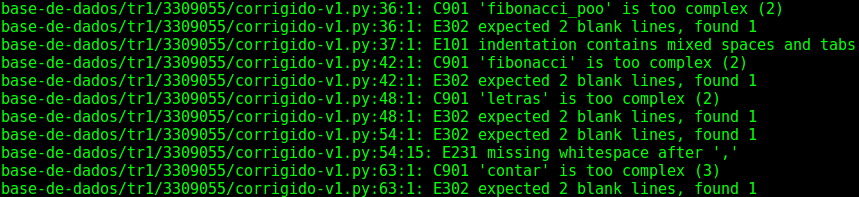
\includegraphics[width=1\linewidth]{imagem/flake8}
			\caption{Representação das características analisadas pelo \texttt{Flake8}}
			\label{fig:flake8}
		\end{figure}
		
		A \cref{fig:flake8} apresenta o formato da impressão de cada característica do
		\texttt{Flake8}. Notamos que era possível obter as características no momento em
		que fosse realizado cada \texttt{print} dos dados, visto que, todas as linhas
		possuem o tipo do erro, E302 ou a complexidade ciclomática C901, por exemplo.
		Desta forma, alteramos o método \texttt{get\_file\_result()} da classe
		\texttt{reporter} do \texttt{Flake8}. Criamos um dicionário contendo todos os
		erros do \texttt{PEP8} e do \texttt{mccabe} como chave. A cada impressão
		verificamos qual é o tipo do erro e incrementamos o valor dessa chave.
		
		\begin{figure}[h]
			\centering
			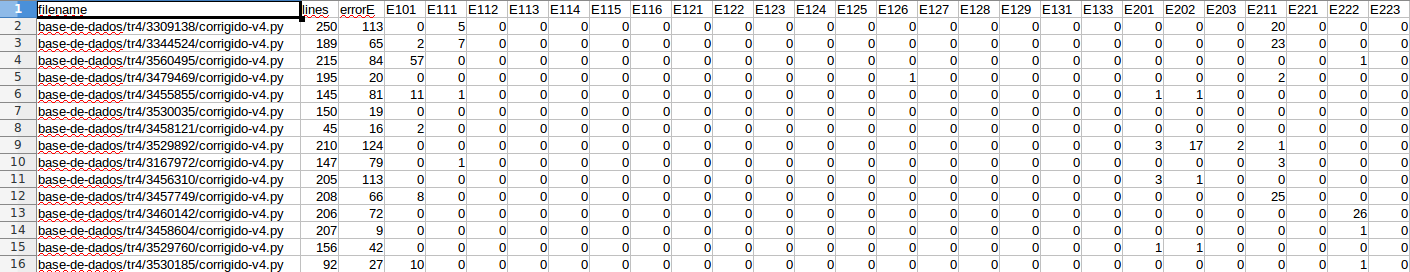
\includegraphics[width=1\linewidth]{imagem/arquivoCSV}
			\caption{Arquivo no formato \texttt{CSV} gerado após as adaptações inseridas nas ferramentas \texttt{Flake8} e \texttt{PEP8}}
			\label{fig:arquivoCSV}
		\end{figure}
		
		A \cref{fig:arquivoCSV} apresenta o arquivo gerado pelas ferramentas após a
		execução das análises de cada código-fonte presente no caminho \texttt{base-de-dados/}.
		As três primeiras colunas são: o nome do arquivo, a quantidade de linhas implementadas
		e o total de erros do estilo de escrita PEP 8 \cite{van2001pep}, respectivamente. As
		demais colunas são referentes a cada erro do \texttt{PEP8} \cite{pep8} com a última
		coluna representando a complexidade ciclomática calculada pela ferramenta
		\texttt{McCabe} \cite{mccabe}.

	\section{Mineração de dados e agrupamento}
		Com a finalidade de encontrar relações entre as características extraídas, em
		conformidade com a etapa Extração de Padrões (\cref{fig:mineracaoDados}).
		Utilizamos a técnica de similaridade do cosseno. Sua escolha ocorreu pelo fato de obtermos
		uma matriz esparsa -- possui grande quantidade de 0 (zeros) -- ao realizar o
		Pré-Processamento (\cref{fig:mineracaoDados}) das características extraídas. A
		ocorrência da grande quantidade de 0 (zeros) ocorre pela busca dos programadores
		em implementar suas soluções computacionais corretamente. Além disso, faz com que
		implementações para problemas distintos não sejam consideram semelhantes devido a
		quantidade de 0 (zeros) nas mesmas características. A grande quantidade de 0 (zeros)
		pode ser observada na \cref{fig:arquivoCSV}.
	
	\section{Projeção e visualização}
		Para possibilitar a visualização dos agrupamentos utilizaremos a \texttt{Science View}
		\cite{Alencar-etal:2012} que utiliza o algoritmo de agrupamento \acs{DBSCAN} \cite{Ester1996}
		e a técnica de projeção multidimensional dinâmica \ac{T-LSP} \cite{Alencar}. Até o momento,
		realizamos a adaptação para leitura do arquivo no formato \texttt{CSV}. A \acs{T-LSP} \cite{Alencar}
		produz uma sequência temporal de mapas conforme a similaridade dos dados. Com isso, poderemos
		verificar se o aluno está progredindo no curso, visto que a técnica de projeção permitirá
		visualizar projeções relativas a implementações por semana ou meses, por exemplo. Desta
		forma, poderemos obter sequências temporais de mapas baseado na similaridade das
		implementações de um único aluno.
		
		% TODO: Marco: escrever sobre como a projeção pode ser utilizada para avaliação de trabalhos: requisitos
		% e instruções com a ScienceView
		
			
		% TODO: indicar que as próximas seções serão sobre a visualização de duas bases
		As duas próximas seções irão descrever a visualização de duas bases de dados
		distintas, descrevendo a base de dados, sua avaliação, a forma que foi realizado
		seu experimento e o resultado qualitativo.
		
	\section{Projeção e visualização de APOO com Python}
	
	\subsection{Descrição da base}
	% TODO: descrever base de dados: quais foram os tipos de programas, quantos foram, falar que a
	% base foi anomizada.
	Essa base é constituída de 152 implementações de 5 problemas distintos. O primeiro exercício
	consiste na revisão de conceitos básicos como: estruturas de condição e laço de repetição. O
	segundo exercício define a criação de classes com mais de um construtor, e manipulação de
	arquivos e cadeia de caracteres. O terceiro exercício consiste na criação das classes
	\texttt{Palavra} e \texttt{Texto}, no qual a primeira classe deve ser utilizada na segunda
	classe, e uma classe para gerar orações gramaticais. O quarto exercício refere-se a
	utilização de herança e polimorfismo, identificando cada palavra contida em um arquivo. E
	o quinto exercício consiste na alteração de uma classe, implementando sobreposição de
	operadores. Os desenvolvedores das implementações foram anonimizados, sendo representado
	por uma sequência de números.
	
	\subsection{Avaliação da projeção com preservação de vizinhança}
	
	
	\subsection{Avaliação qualitativa da visualização}
	% TODO: relatar o estudo: treinamento, instruções, questionário, resultados
	
	
		\begin{figure}[h]
			\centering
			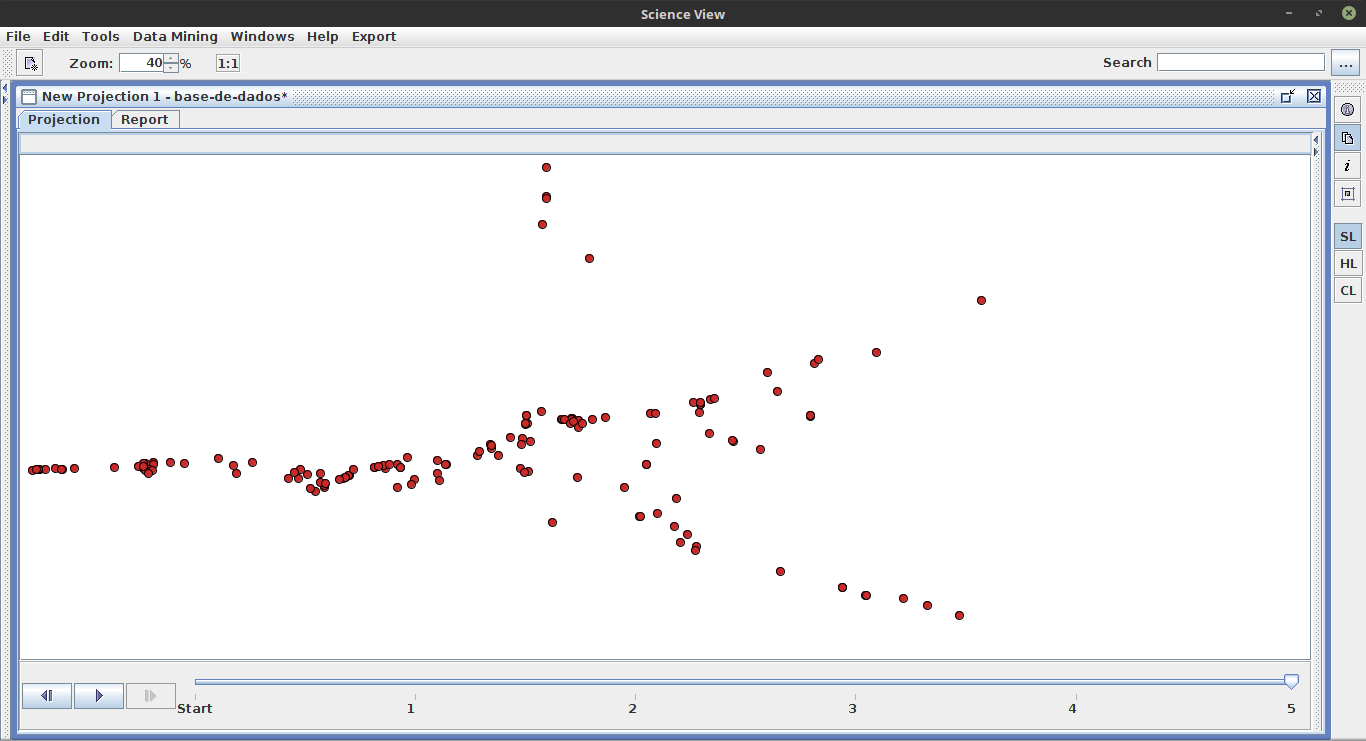
\includegraphics[width=1\linewidth]{imagem/projecaoFinal} % TODO: substituir, futuramente, pela figura da ferramenta corrigida.
			\caption[Visualização dos agrupamentos da base de dados gerado pela \texttt{Science View}]
			{Visualização dos agrupamentos da base de dados gerado pela \texttt{Science View} \cite{Alencar-etal:2012}}
			\label{fig:projecaoFinal}
		\end{figure}
		
		A \cref{fig:projecaoFinal} apresenta a visualização dos agrupamentos das 152
		implementações contidas na base de dados. Isso foi possível após a adaptação da
		ferramenta para leitura de arquivos no formato \texttt{CSV}. Cada ponto da
		visualização é referente a um código-fonte. Ao clicar em um dos pontos, a
		\cref{fig:codigo1} mostra a exibição da sua implementação e
		as características extraídas das ferramentas para aquele código-fonte. Também
		é possível ordenar a coluna de características \foreign{Quantity} em ordem
		decrescente para visualizar as características que mais ocorreram.
		
		As implementações das \cref{fig:codigo1} e \cref{fig:codigo2} foram consideradas
		semelhantes, devido aos seus respectivos pontos estarem próximos no mapa de
		projeção. Ao ordenarmos a coluna \foreign{Quantity} é possível notar que há
		diversas semelhanças nos tipos das características extraídas e erros que
		ocorreram, além da quantidade dessas características.
		
		\begin{figure}[h]
			\centering
			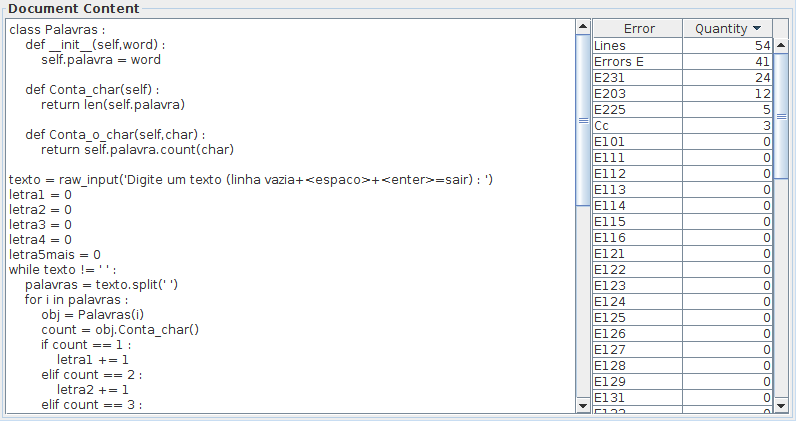
\includegraphics[width=0.8\linewidth]{imagem/codigo1}
			\caption[Representação parcial da interface que apresenta o código e suas características]
			{Representação parcial da interface que apresenta o código e suas características \cite{Alencar-etal:2012}}
			\label{fig:codigo1}
		\end{figure}
		
		\begin{figure}[H]
			\centering
			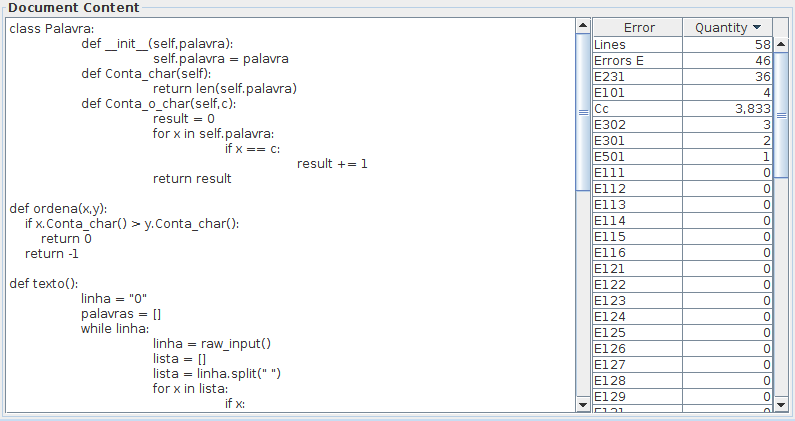
\includegraphics[width=0.8\linewidth]{imagem/codigo2}
			\caption[Representação parcial da interface que apresenta o código considerado semelhante ao da \cref{fig:codigo1}]
			{Representação parcial da interface que apresenta o código considerado semelhante ao da \cref{fig:codigo1} \cite{Alencar-etal:2012}}
			\label{fig:codigo2}
		\end{figure}


	% TODO recomendo a colocação de uma imagem da curva de neihborhood  preservation para uma de suas projeções na seção resultados.
	
	
	\section{Projeção e visualização de MIT 6.00.1x}	

	\subsection{Descrição da base}
	% TODO: descrever base de dados: quais foram os tipos de programas, quantos foram, falar que a
	% base não foi anonimizada porque os programas estavam publicamente disponíveis no GitHub.
	Essa base de dados é constituída de 3470 implementações referente a 10 exercícios
	distintos. Todos as atividades solicitam manipulação de arquivo e cadeia de caracteres.
	
	O primeiro exercício requer conceitos de matriz, utilizando lista dentro
	de lista, e programação dinâmica para solucionar o transporte de animais.
	
	O segundo exercício necessita de conhecimento sobre aleatoriedade, lista, condicional,
	cadeia de caracteres, operações aritméticas e lógicas para implementar o jogo da
	forca.
	
	O terceiro exercício solicita a utilização de laço de repetição, condicional, lista,
	operações aritméticas e lógicas para implementar o jogo das palavras.
	
	O quarto exercício requer conhecimento de lista e dicionário pra codificar e
	decodificar um texto.
	O quinto exercício requer o uso de analisador (\foreign{parser}), construção
	de classe, interface, polimorfismo e operadores lógicos para desenvolver um programa
	de monitoramento de novos \foreign{feeds} na Internet.
	
	O sexto exercício solicita conhecimento sobre criação de classes, matriz, laço de
	repetição e manipulação de interface gráfica para implementar um aspirador de pó
	inteligente e sua simulação.
	
	O sétimo exercício consiste no uso de classes, aleatoriedade, laço de repetição,
	condicional, lista e conhecimento de estatística para implementar uma simulação
	e um sistema de tratamento de pacientes conforme o vírus que eles possuem.
	
	O oitavo problema consiste na implementação de classes a partir do exercício $7$.
	Pedindo a implementação da classe \texttt{ResistantVirus} e \texttt{SimplePatient}
	para realizar simulações desses vírus em pacientes.
	
	O nono exercício requer o uso de dicionário e operador lógico para desenvolver
	um software que apresente uma lista de assuntos para cada aluno da universidade.
	
	E para o décimo exercício, é necessário conhecer um algoritmo de agrupamento para
	realizar sua implementação.
	
	Os desenvolvedores dessas implementações não foram anonimizados, pois seus
	códigos-fontes estavam presentes em repositórios públicos no GitHub \cite{github}.
	
	% TODO: Marco: colocar a string utilizada para buscar os programas e como foi criada a base
	

\subsection{Avaliação da projeção com preservação de vizinhança}


\subsection{Avaliação qualitativa da visualização}
% TODO: relatar o estudo: treinamento, instruções, questionário, resultados



	\section{Considerações finais}
	
		O atual banco de dados de implementações, formado por 152 códigos-fontes que
		solucionam 5 problemas distintos é considerado pequeno e pode enviesar o
		projeto. Para isso, construiremos outro banco de dados de implementações
		por meio de submissões de voluntários, visando possuir um conjunto de
		implementações vasto para a pesquisa.
